\section{Algorithm}\label{sec:optimization}

\comments{
Assuming every face in the carton model is rigid, which means the interior angle in each plane stays the same.  
%
Furthermore, planes are connected by hinges at the boundary of patches, and the planar layout has its front and back.}

In this section, we explain our algorithm in detail. 
Initially, assume that the 2D layout $L$ lies on the $XOY$ plane, so that each vertex $\mathbf{v}_i=(x_i,y_i,z_i)$ in $V$ has $z_i=0$. 
Each face in $F$ has a normal $\mathbf{n}_i=(0,0,1)^T$.
%
In the first step of our algorithm, our system automatically {\color{blue}{folds the original flat mesh into a rough model by assigning a specific angle to each fold edge.}}
%computes the normal of the desired 3D carton based simple rules of orthogonality and parallelism.
In the second step, the carton shape is refined based on a set of possible geometric constraints.



%\cxj{re-write this section. Describe clearly about the parameters, the objective, and methods. }
%In this section we explain the reason why using a specific angle to each fold edge, and constructing our initialized model. 

A general process for humans to fold a carton starts from folding each edge by a rough angle and then connecting close vertexes to obtain a box-like shape. 
Naturally, we first fold the 2D layout by assigning a rotation angle to each pair of adjacent faces to get a rough shape, instead of directly computing the vertex coordinates.
%The basic idea is to interpret the folded state of a box as a series of rotation angles along each edge, and by setting specific value of angles which is $\pi/2$, we can have a rough model to assist the later optimization.
%	
Observed from existing data in the Internet, most of the traditional cartons are cuboid for holding files or delivering daily supplies. 
Although there is a recent trend to design more complicated layouts to attract consumers, the shape of these unusual cartons is similar to boxes as their functions are still packaging commodity. 
%
Therefore, we choose $\pi/2$ as the initial value of the rotation angle to each folding edge. 
%
First, a face graph of a layout is constructed, as shown in Figure~\ref{fig:midresult} (a).
Each face is a node, and there is an edge between two faces if they are connected by a folding edge.
%
The faces in the 2D layout are recursively folded in a breadth-first manner.
Starting from the face with the maximal area, our system folds all its adjacent faces by rotating them around their connecting edge by $\pi/2$, and then continues to others. 
Figure~\ref{fig:midresult} illustrates the folding process of a cuboid carton. 

\begin{figure}[ht]
	\centering
	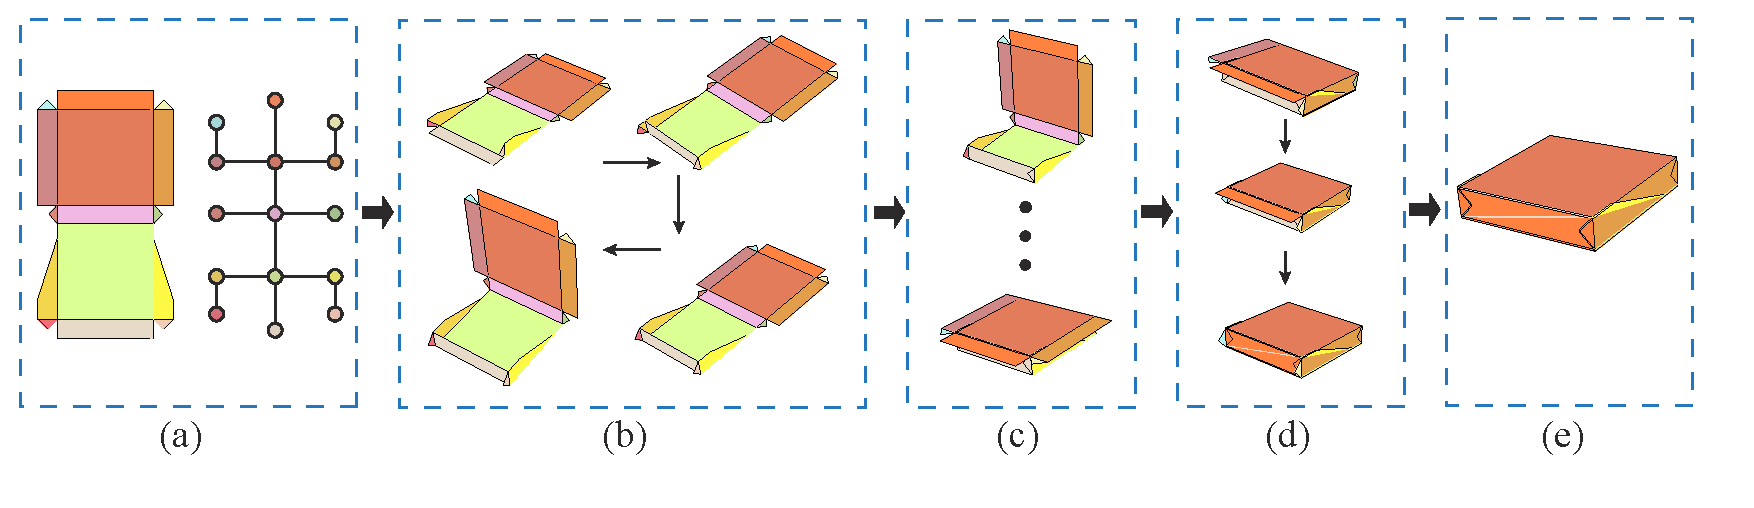
\includegraphics[width=0.9\textwidth]{images/midresult}
	\caption{A rough 3D shape is obtained by folding each face by $\pi/2$ in the 2D layout (a) in a breadth-first manner, starting from the face with the maximal area. (b), (c), (d) and (e) are the different folding stages in the initialization step.}
	\label{fig:midresult}
\end{figure}


{\color{blue}{The following two figures}} shows a group of results generated by simply folding faces by $\pi/2$.
Traditional cartons in cuboid shapes could reach an ideal state, as Figure~\ref{fig:initial-automatic} shows.
However, many complicated designs still need refinement, such as the four examples in Figure~\ref{fig:initial-need-improvement}. 
Take the hexagonal box as an example, the 3D model can be improved by simply snapping the small paste faces to its nearby faces. %
%
As a result, we provide an suggestive interface by automatically detecting potential geometric modifications in the rough carton shape for users to explore.
%interactively allow users to add these constrains into our system and optimize to a desired model, as described in the following section.

\begin{figure}
	\centering
	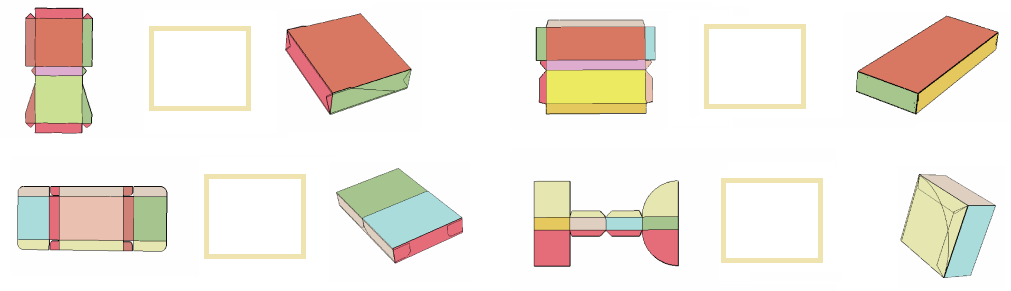
\includegraphics[width=0.9\textwidth]{images/initial-auto.png}
	\caption{Four examples of carton models that can be fully automatically generated from 2D layouts by folding each edge with a fixed angle $\pi/2$. }
	\label{fig:initial-automatic}
\end{figure}


\begin{figure}
	\centering
	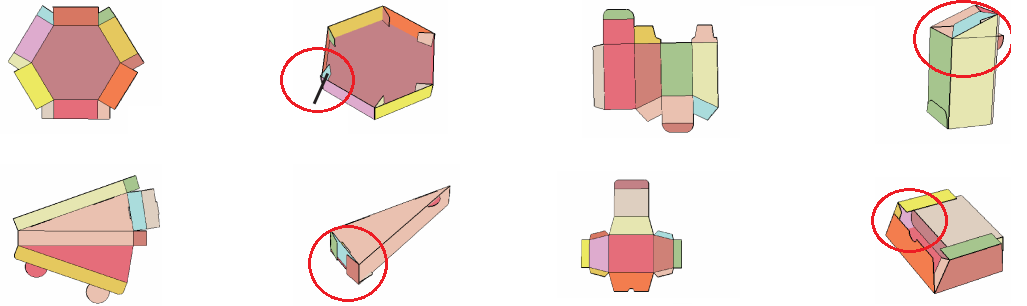
\includegraphics[width=0.9\textwidth]{images/initial-improve.png}
	\caption{Four examples of the carton models that need shape improvement. While the shapes are not cuboid, using a fixed angle $\pi/2$ leads to non-closed shape and loose structure. }
	\label{fig:initial-need-improvement}
\end{figure}
%%%%%%%%%%%%%%%%%%%%%%%%%%%%%%%%%%%%%%%%%%%%%%%%%%%%%%%%%%%%%%%%%%%%%


\cxj{It is not clear how do you assign the angle $\pi/2$ to all angles. What order do you use? Show the mid-stage? any problem need to discuss? }

\subsection{Shape Refinement}\label{sec:refinement}

%there is still a need to refine the results that have not folded into pleasing results. 
Though not perfect, the initial 3D shape provides a good start point for generating the final carton model. 
%
To further refine the 3D shape, the 3D coordinates of all the vertexes are then computed based on a set of shape constraints.
%
%the main idea is to prescribe the shape constrains by a set of vertexes of the polymesh. 
Moreover, with the extra information acquired from user interaction, we can finally construct the desired 3D realization.
In this step, the coordinate of vertexes are chosen as our objective instead of angles on folding edges.
This is mainly because that the geometric constrains in the 3D shape can be more simply and intuitively represented by 3D vertexes.
% and we can implement the algorithm introduced by Bouaziz et al. easily~\cite{Bouaziz:2012:SSD:2346796.2346802}.
 

%\subsection{Aided Detection}

%While the initial 3D model with simple angle folding provides a rough idea about the carton shape, 
Our system  automatically detects a group of possible shape constraints to form the final 3D model, such as vertex merging, shape symmetry, and so on. 
%
These guiding operations are provided to the user at bottom of the user interface, for the user to quickly select and explore the carton shapes.
In our system, \cxj{two} types of shape refinement operations, vertex merging, and shape symmetry, are automatically detected.

%
%In order to assist users construct the final carton interactively, we also provide symmetry detection and merging points detection to improve the efficiency of constructing models .

\noindent
\textbf{Vertex merging} is detected among the nearby vertexes. 
For irregular shapes consists of non-rectangular faces or non-perpendicular adjacent faces, some vertexes supposed to folded to the same position are close to each other after the initialization step. 
For each pair of vertexes $\mathbf{v}_a$, $\mathbf{v}_b$ {\color{blue}{that in the nonadjacent face}}, if $|\mathbf{v}_a-\mathbf{v}_b|<\epsilon$, and one edge connecting to $\mathbf{v}_a$ has the same length with one edge connecting to $\mathbf{v}_b$.
\cxj{Add discussion about more than two vertexes. Improve figure by highlighting the merging edge and vertex. }
{\color{blue}{While there are sometimes more than two vertexes that need to be merged, as an example shown in Figure~\ref{fig:suggestion} (a), after $\mathbf{v}_a$ and $\mathbf{v}_b$ being considered to relocate in the same place, if the next vertex $\mathbf{v}_c$} is detected satisfying $|\mathbf{v}_c-\mathbf{v}_a(\mathbf{v}_b)|<\epsilon$ and one of incident edges of $\mathbf{v}_c$ has the same length as $\mathbf{v}_a(\mathbf{v}_b)$'s, vertex $\mathbf{v}_c$ also has the need to merge with $\mathbf{v}_a$ and $\mathbf{v}_b$.}

%Consider the initialization results can represent the ideal model partly, the disadjacent vertices that have one edge with same length can be regarded as targets that need to be located in the same place if their Euclidean distance is below a certain threshold.

\noindent
\textbf{symmetry detection} {\color{blue}{focus on the symmetry property of vertexes. $\mathbf{v}_a$ and $\mathbf{v}_b$ are regarded as symmetric pair, if for each pair of $l_{ai} \in \{ l_{a1},l_{a2}...l_{am}\}$ and $l_{bi} \in \{ l_{b1},l_{b2}...l_{bn}\}$, $m = n$ and $|l_{ai}- l_{bi}|<\epsilon$ where $m$ is the number of $\mathbf{v}_a$'s ordered set of the incident edges' length $\{ l_{a1},l_{a2}...l_{am}\}$, and $n$ is the number of $\mathbf{v}_b$'s ordered set of the incident edges' length $\{ l_{b1},l_{b2}...l_{bn}\}$.
		
 When involving multiple vertexes, the searching criterion is based on symmetric vertex pair detection described above. The symmetric vertex set of selected vertexes $\{\mathbf{v}_1,\mathbf{v}_2,...,\mathbf{v}_{n-1}\}$ is $\{\hat{\mathbf{v}}_1,\hat{\mathbf{v}}_2,...,\hat{\mathbf{v}}_{n-1} \}$, the vertex set $\{\mathbf{v}_1,\mathbf{v}_2,...,\mathbf{v}_n\}$ has the symmetric vertex set $\{\hat{\mathbf{v}}_1,\hat{\mathbf{v}}_2,...,\hat{\mathbf{v}}_n \}$, if $||\mathbf{v}_n-\mathbf{v}_i| - |\hat{\mathbf{v}}_n-\hat{\mathbf{v}_i}||<\epsilon$, for $i = 1,....,n-1$.}} 

%On account of the simplicity of the carton shape, the vertexes that have same length set of incident edges can be regarded as symmetric pair. While users select vertexes that need to be merged together, symmetry detection can reduce repetitive work by giving users suggestions of symmetric vertexes.
\cxj{Describe your algorithm first. Then explain fig 5 as a specific example.}

\cxj{Add a figure to illustrate this. }
{\color{blue}{Take Figure~\ref{fig:suggestion} (b) as an example, after users selecting vertexes circled in red, our system can automatically detect their symmetric set circled in blue. As an result, our system can detect these symmetry pairs to assist users improve efficiency.}}

\begin{figure}
	\centering
	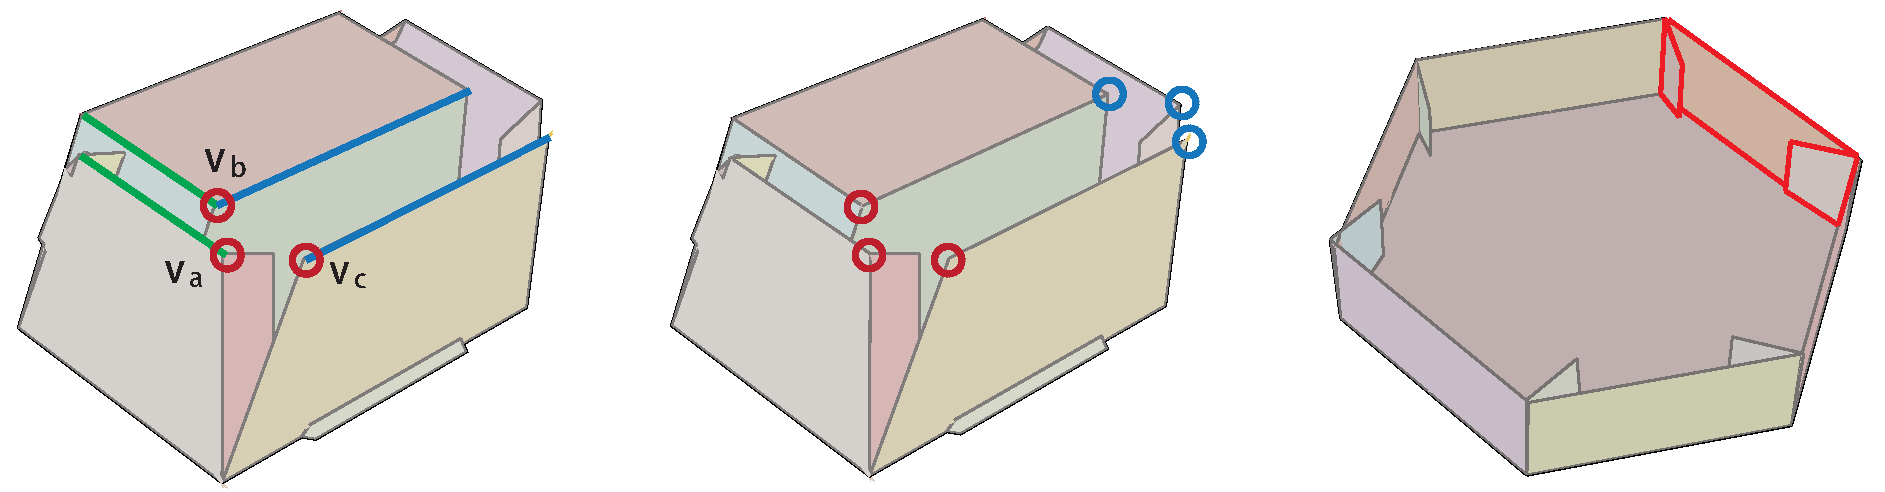
\includegraphics[width=0.9\textwidth]{images/suggestion}
	\caption{Vertex merging detection is well illustrated by (a), $\mathbf{v}_a$ and $\mathbf{v}_b$ may have the need to merge cause $|\mathbf{v}_a-\mathbf{v}_b|<\epsilon$, and one edge connecting to $\mathbf{v}_a$ marked as green has the same length with one edge connecting to $\mathbf{v}_b$ also marked as green. $\mathbf{v}_c$ can also be considered that need to merge with $\mathbf{v}_a$ and $\mathbf{v}_b$ as $|\mathbf{v}_c-\mathbf{v}_a(\mathbf{v}_b)|<\epsilon$ and one of incident edges of $\mathbf{v}_c$ marked as blue has the same length as $\mathbf{v}_a(\mathbf{v}_b)$'s also marked as blue. While users select three vertexes circled in red (b), our system can detect symmetric vertexes circled in blue automatically. \cxj{show more possible suggestions in this figure. Make sure the font in consistent with the caption}.\cxj{the font of a, b is too big. Is this automatically detected result?}}
	\label{fig:suggestion}
\end{figure}

\cxj{Once the user selects a suggested shape refinement operation, we optimize the 3D shape based on a series of geometric constraints.}
%We now introduce the constrains used in our construction method:
Given the current mesh whose vertex positions are defined as $\{\vo_i\}^{N}_{i=1}$, a new mesh with the same topology but new vertex positions $\{\vn_i\}^{N}_{i=1}$ is constructed.
%
The geometric constraints can be classified into two groups, basic geometric constraints and user-selected constraints. 
First, to keep the geometric shape of each face, the constraints including edge length constraint, coplanarity, and face rigidity, which are corresponding to similarity constraint and plane constraint described in \cite{Bouaziz:2012:SSD:2346796.2346802}. 

\noindent
\textbf{Edge length constraint} 
For each edge $\{e_j\}_{j=1...M}$, its length should be preserved when refine the carton shape.
Hence, its two endpoints $\mathbf{v}_{js}$ and end point $\mathbf{v}_{jt}$ should satisfy 
\begin{equation}
||\mathbf{v}_{js} - \mathbf{v}_{jt}||^2 = ||\mathbf{\hat{v}}_{js} - \mathbf{\hat{v}}_{jt}||^2.
\label{equ:edge}
\end{equation}
%to ensure that the length of each edge stays the same.

\noindent
\textbf{Coplanarity} {\color{blue}{For each face $\{p_k\}_{k=1 \dots P}$, this constraint specifies the face's vertexes should always lie on a plane. We can compute the sorted eigenvectors $\mathbf{U} = [\mathbf{e}_1, \mathbf{e}_2, \mathbf{e}_3]$ of the $ 3 \times 3$ covariance matrix $\mathbf{C}^T\mathbf{C}$ where $\mathbf{C} = \{\mathbf{v}_{kj}\}_{j=1}^{N_k}$, $\mathbf{v}_{kj}$ is the $j$th vertex among $N_k$ vertexes in face $p_k$}. Plane projection can be obtained by removing the last column of $\mathbf{U}$. }
%For each face $\{p_k\}_{k=1 \dots P}$ and its normal $\mathbf{n}_k$, each line connected by two points $\mathbf{v}_{ka}, \mathbf{v}_{kb}$ on the plane is perpendicular to the normal. 
\cxj{where do you get the face nornal in the refined shape?}

\noindent
\textbf{Face rigidity} For each face $\{p_k\}_{k=1 \dots P}$, the length of each line connecting two non-adjacent points $\mathbf{v}_{ka}, \mathbf{v}_{kb}$ on the plane remains the same, so that the shape of each plane keeps unchanged.
\begin{equation}
||\mathbf{v}_{ka} - \mathbf{v}_{kb}||^2 = ||\hat{\mathbf{v}}_{ka} - \hat{\mathbf{v}}_{kb}||^2.
\label{equ:plane}
\end{equation}

The information acquired from user interaction will add enough constrains to solve the optimization problem, and one of the interaction is to choose the right given suggestion including points needed to be merged together. As for the point information, the constrains can be written like:

\noindent
\textbf{Merging vertexes} For any two vertexes $\mathbf{v}_p$ and $\mathbf{v}_q$ that are selected to be merged as the same vertex, we have 
\begin{equation}
\mathbf{v}_p - \mathbf{v}_q = 0.
\label{equ:point}
\end{equation}
%if these two points $\mathbf{v}_p$, $\mathbf{v}_q$ need to be moved into the same place.
\cxj{shape symmetry?}


When the above constrains still lead to an ill-posed problem, soft constraints will be added to keep the original positions of irrelevant vertexes. 


\noindent
\textbf{Irrelevant vertexes} $\{\mathbf{v}_i\}$ which are not in the same plane with $\mathbf{v}_p$ or $\mathbf{v}_q$, should be stay at their original location. 
We add these soft constraints by adding a small weight $w$, which is set 0.001 in our experiments. 
\begin{equation}
\mathbf{v}_i - \mathbf{\hat{v}}_i = 0.
\label{equ:irrelevant}
\end{equation}

Figure~\ref{fig:constrain} illustrates the necessity of basic three constrains.
\cxj{More detailed explaination on the figure. Explain the three constraints in the figure.}
{\color{blue}{When we merge three vertexes circled in red Figure~\ref{fig:constrain} (b) into one location, the optimized model is generated under basic constraints shown in Figure~\ref{fig:constrain}}. The model shown in Figure~\ref{fig:constrain} (d) (e) and (f) are the results after optimizing without edge length constrain, coplanarity and face rigidity constrain separately. Without edge length constrain, the two red edges have been stretched Figure~\ref{fig:constrain} (d), the face surrounded by red lines Figure~\ref{fig:constrain} (e) is not a standard plane without coplanarity, and the face surrounded by red lines in Figure~\ref{fig:constrain} (f) has been deformed without face rigidity.}

\begin{figure}
	\centering
	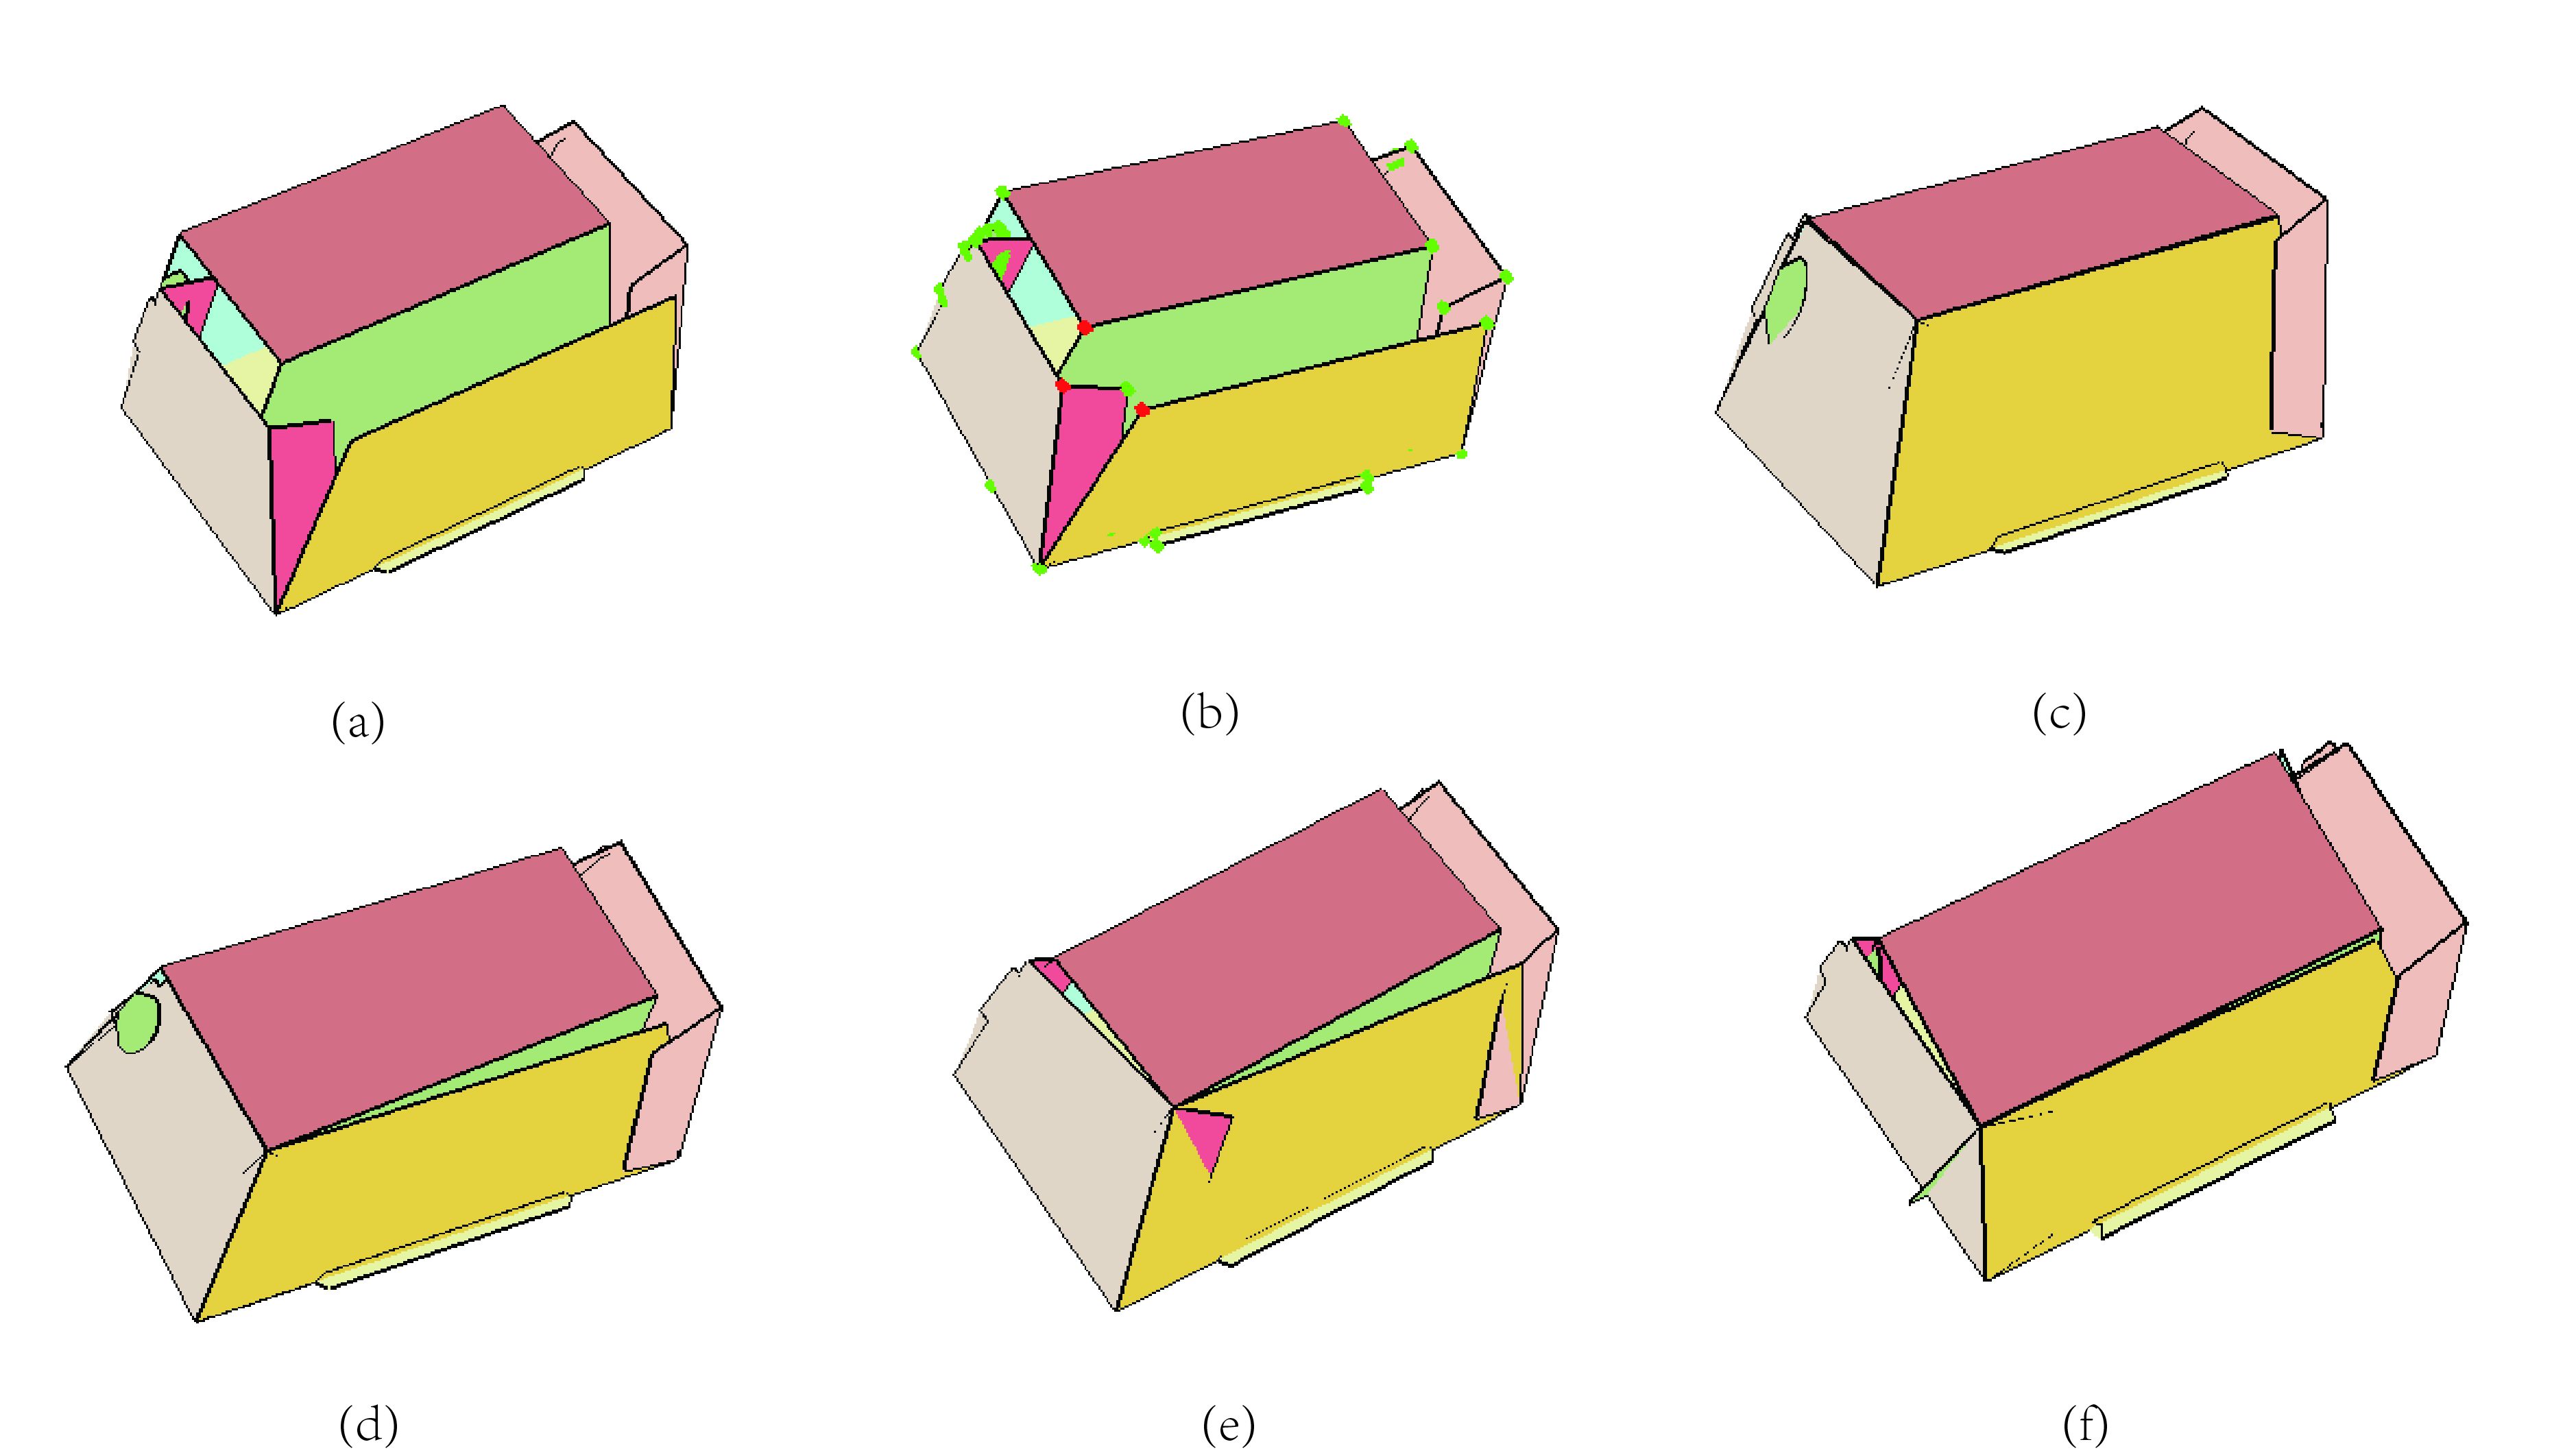
\includegraphics[width=0.9\textwidth]{images/constrain.jpg}
	\caption{Given an initial state~(a), by choosing three points marked in red~(b) that need to be relocated together, basic three shape constrains can lead to the optimization result~(c). The bottom three are the results optimized lack of edge length constrain, coplanarity and face rigidity separately, compared to~(c), the results can not keep the basic shape well. Without edge length constrain, the two red edges have been stretched (d), the face surrounded by red lines (e) is not a standard plane without coplanarity, and the face surrounded by red lines in (f) has been deformed without face rigidity.}
	\label{fig:constrain}
\end{figure}

